\chapter{Experiments and Results}
\label{chapter:experiments}

So far we have discussed the CCD approach in detail. In this chapter,
the experimental evaluation of the CCD algorithm and the naive CCD tracker will be provided. In previous
chapter, we have introduced the application of the CCD algorithm and
its variant. Experiments have been performed on the PR2. we apply the
CCD approach to three different kinds of model fitting and tracking
problems:

\begin{enumerate}
\item Contour convergence on still image
\item Tracking initialization from sift features
\item Tracking initialization from 3D point cloud
\end{enumerate}

We analyze the performance of the approach in terms of robustness,
accuracy and runtime. This is followed the comparison between the CCD
approach and  other state-of-the-art methods.
% by the experimental evaluation of the CCD
% algorithm. presents the evaluation of the naive CCD
% tracker and 

\section{Contour convergence on still image}
\label{sec:ES}

As mentioned in related work, the CCD algorithm is an effective
segmentation method like other model-based segmentation algorithms.

A segmentation of an image $I: \Omega \subset R^2 \longrightarrow R$
is the partitioning of its domain into homogeneous regions
$\Omega_1,\ldots, \Omega_n \subset \Omega$. There are many pratical
applications of image segmentation, such as medical imaging, object
tracking, face recognition, fingerprint recognition, machine vison and
so on. In this thesis, we concern its application in object tracking.
In many cases segmentation is the bottleneck when trying to tracking a
object. Many segmentation methods are developed, however, there is not
general solution to the segmentation problem. In the real world,
segmentation problems will often require much domain knowledge before
a successful segmentation can be performed. The CCD algorithm is just
such a method which is combined with the prior knowledge. By
converting a pure segmentation problem to a problem in pattern
recognition, a large amount of techniques in the field of pattern
recognition are introduced to solve segmentation problems, which are
proved to be effective and helpful. Compared with other segmentation
methods, such as intensive-based method,  cluster method, region-based
method and compression-based methods, the CCD algorithm has following
advantages:
\begin{itemize}
\item restrict segmentation problem to a limited explicit region, it is helpful
  to decrease the computation cost.
\item probabilistic representation of the variation of the registered
  samples could be easily given, thus statistical inference between
  the model and the image will be applied. All these are helpful to
  improve the segmentation results.
\item The CCD algorithm achieves sub-pixel accuracy and high
  robustness because only a relatively small fraction of the pixels is
  taken into account in the end of iteration.
\end{itemize}

In the following, we apply the proposed CCD algorithm to 4 kind of
objects:
\begin{enumerate}
\item segmentation of a ball
\item segmentation of 3-D object
\item segmentation of a transparent object
\item fitting a deformable models
\end{enumerate}

\subsection{Segmenation of a ball}
\label{sec:sb}
Like other model-based method, we model a contour of the ball as the
prior knowledge. Due to existing general contour for spherical object,
besides manual initialization, we can use some built-in function in
OpenCV library to generate the contour with given center and
radius. According the definition of prior distribution, it is required
to guarantee that the hypothesis is in the range of the variation of
registered sample, namely, the initial contour can not be too far away
from the target.

\begin{figure} 
  \begin{minipage}[t]{0.45\linewidth} 
    \centering 
    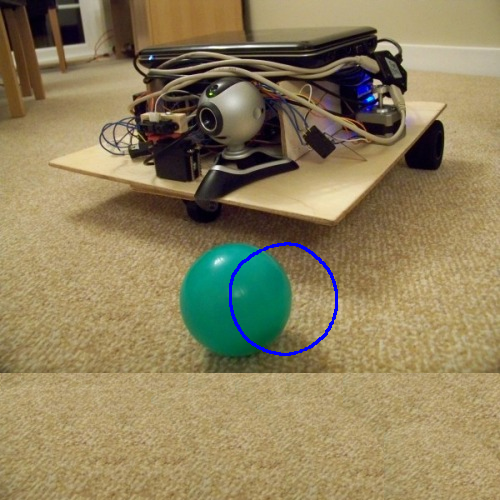
\includegraphics[width=2.0in]{images/ball/0.png} 
    \caption{iteration 1} 
    \label{fig:side:a} 
  \end{minipage}% 
  \begin{minipage}[t]{0.45\linewidth} 
    \centering 
    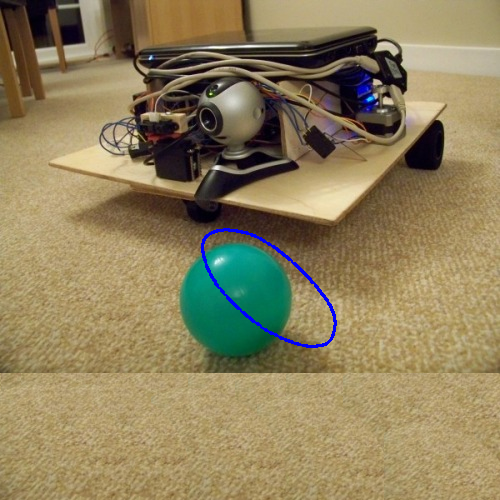
\includegraphics[width=2.0in]{images/ball/2.png} 
    \caption{iteration 3} 
    \label{fig:side:b} 
  \end{minipage} 
  \begin{minipage}[t]{0.45\linewidth} 
    \centering 
    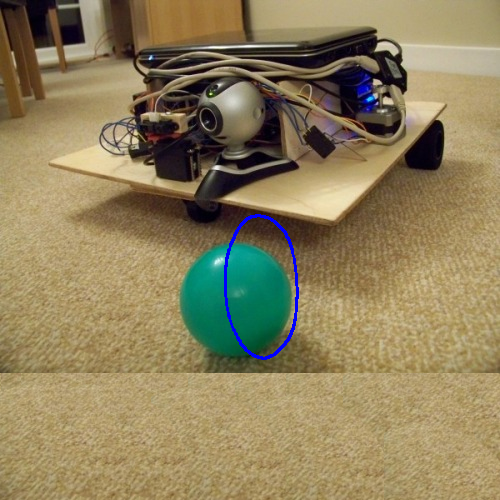
\includegraphics[width=2.0in]{images/ball/6.png} 
    \caption{iteration 7} 
    \label{fig:side:c} 
  \end{minipage} 
  \begin{minipage}[t]{0.45\linewidth} 
    \centering 
    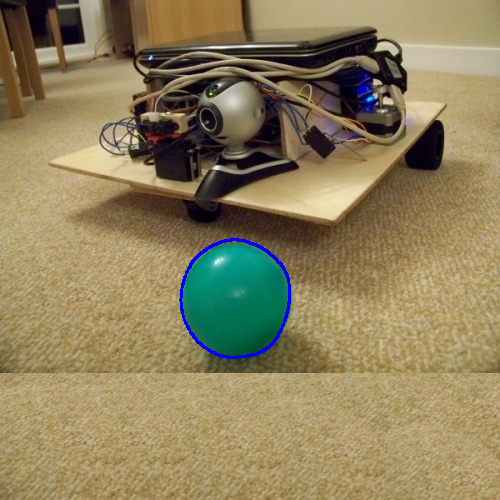
\includegraphics[width=2.0in]{images/ball/15.png} 
    \caption{iteration 16} 
    \label{fig:side:d} 
  \end{minipage} 
\end{figure}

In figure ????, we intentionally give a hypothesis which is far away
from the ball, but after about 15 iteration, we successfully fit the
contour the edge of the ball. For the sake of a ground truth we need
investigate the pixels used in the iterations.

\begin{figure} 
  \begin{minipage}[t]{0.45\linewidth} 
    \centering 
    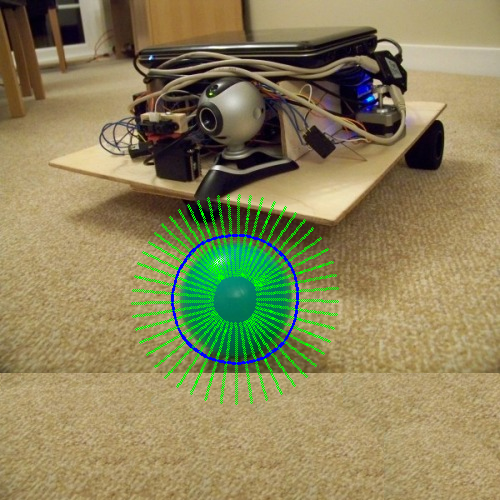
\includegraphics[width=2.0in]{images/ball_normal/0.png} 
    \caption{iteration 1} 
    \label{fig:side:a} 
  \end{minipage}% 
  \begin{minipage}[t]{0.45\linewidth} 
    \centering 
    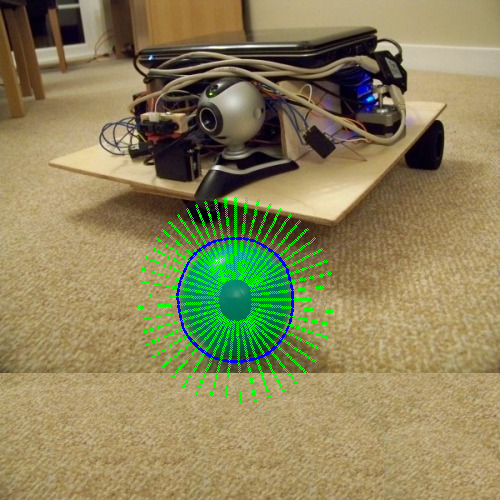
\includegraphics[width=2.0in]{images/ball_normal/1.png} 
    \caption{iteration 2} 
    \label{fig:side:b} 
  \end{minipage} 
  \begin{minipage}[t]{0.45\linewidth} 
    \centering 
    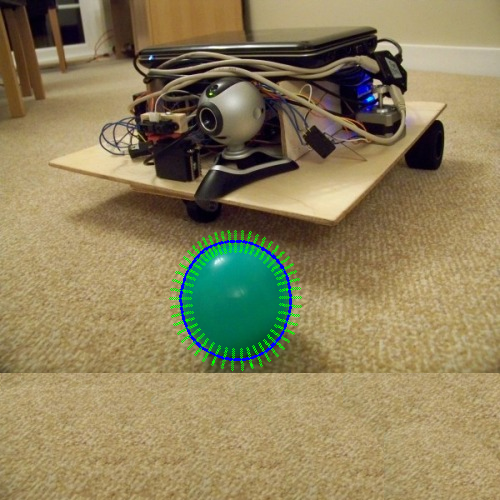
\includegraphics[width=2.0in]{images/ball_normal/3.png} 
    \caption{iteration 4} 
    \label{fig:side:c} 
  \end{minipage} 
  \begin{minipage}[t]{0.45\linewidth} 
    \centering 
    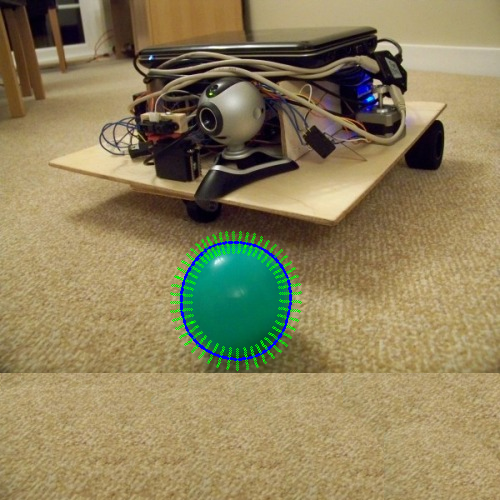
\includegraphics[width=2.0in]{images/ball_normal/4.png} 
    \caption{iteration 5} 
    \label{fig:side:d} 
  \end{minipage} 
\end{figure}



\subsection{Segmenation of a 3-D obejct}
\label{sec:s3o}

\begin{figure} 
  \begin{minipage}[t]{0.45\linewidth} 
    \centering 
    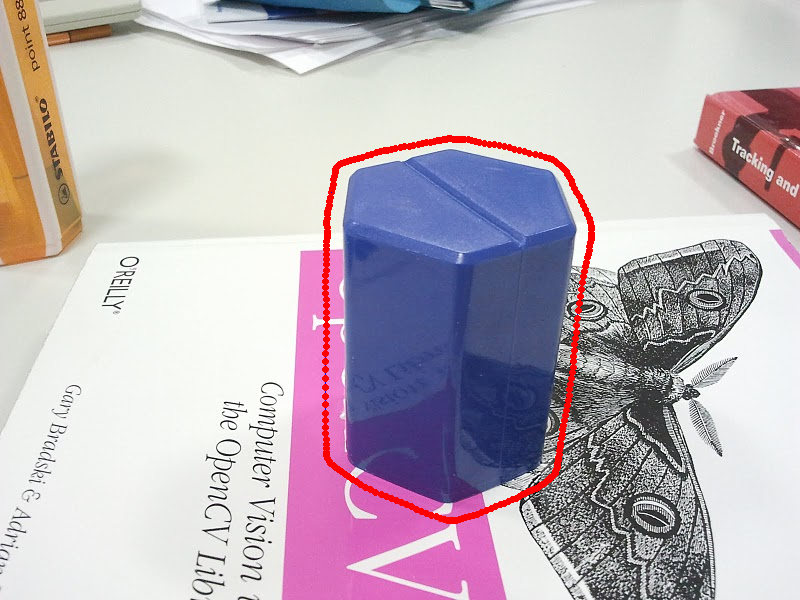
\includegraphics[width=2.0in]{images/container/0.png} 
    \caption{iteration 1} 
    \label{fig:side:a} 
  \end{minipage}% 
  \begin{minipage}[t]{0.45\linewidth} 
    \centering 
    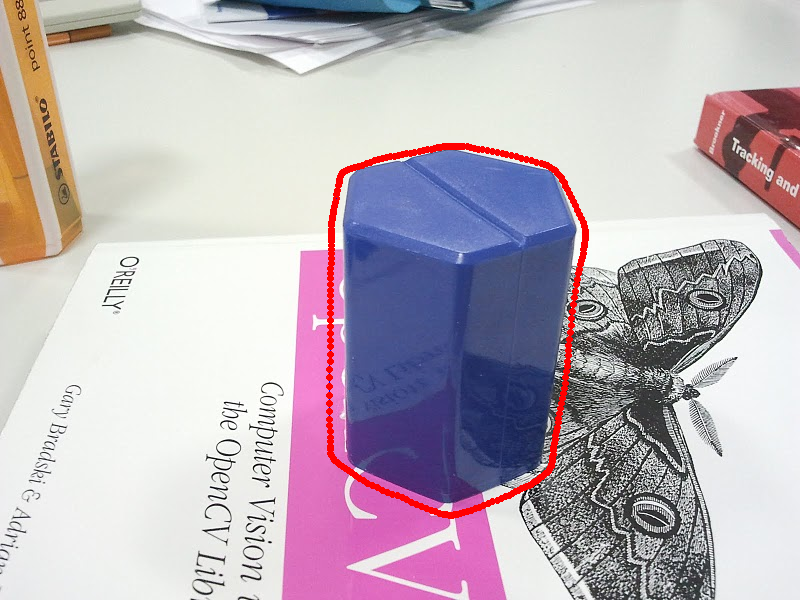
\includegraphics[width=2.0in]{images/container/1.png} 
    \caption{iteration 2} 
    \label{fig:side:b} 
  \end{minipage} 
  \begin{minipage}[t]{0.45\linewidth} 
    \centering 
    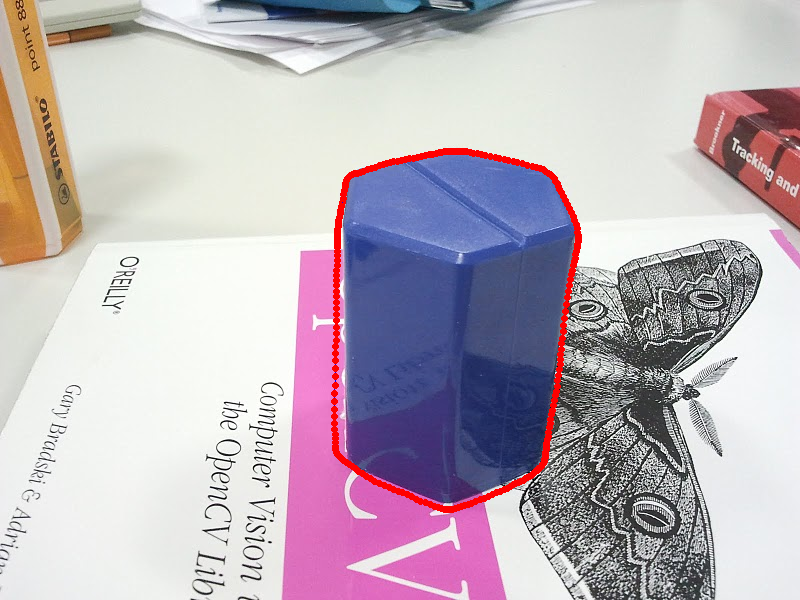
\includegraphics[width=2.0in]{images/container/2.png} 
    \caption{iteration 3} 
    \label{fig:side:c} 
  \end{minipage} 
  \begin{minipage}[t]{0.45\linewidth} 
    \centering 
    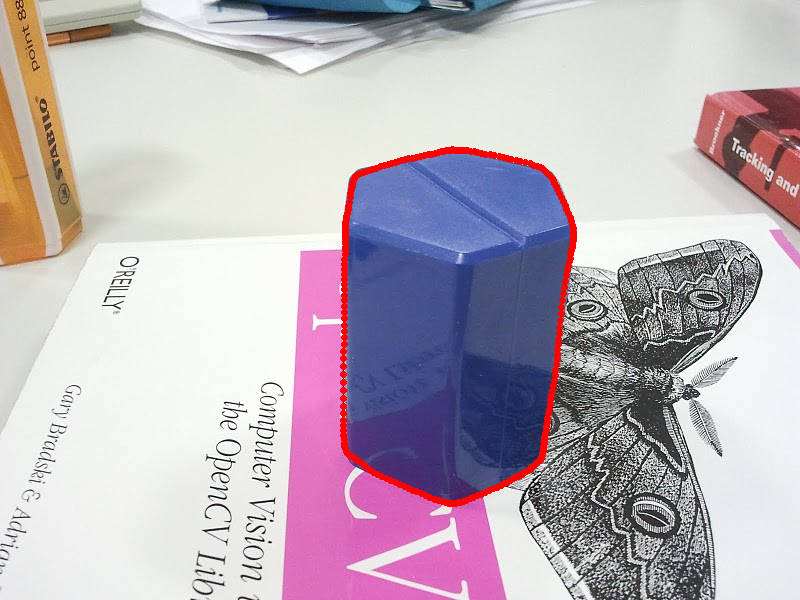
\includegraphics[width=2.0in]{images/container/5.png} 
    \caption{iteration 6} 
    \label{fig:side:d} 
  \end{minipage} 
\end{figure}

\subsection{Segmenation of a transparent obejct}
\label{sec:sto}

\subsection{Fitting a deformable object}
\label{sec:fdo}
\begin{figure} 
  \begin{minipage}[t]{0.45\linewidth} 
    \centering 
    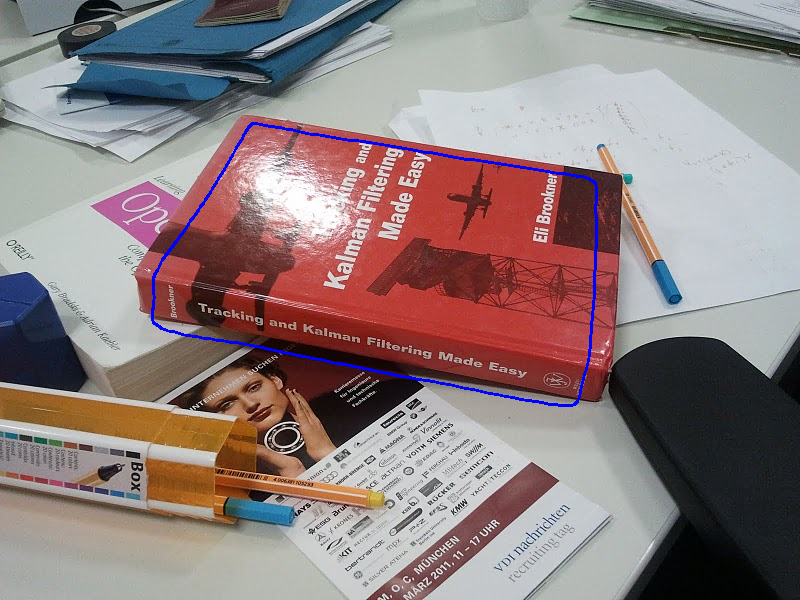
\includegraphics[width=2.0in]{images/book/0.png} 
    \caption{iteration 1} 
    \label{fig:side:a} 
  \end{minipage}% 
  \begin{minipage}[t]{0.45\linewidth} 
    \centering 
    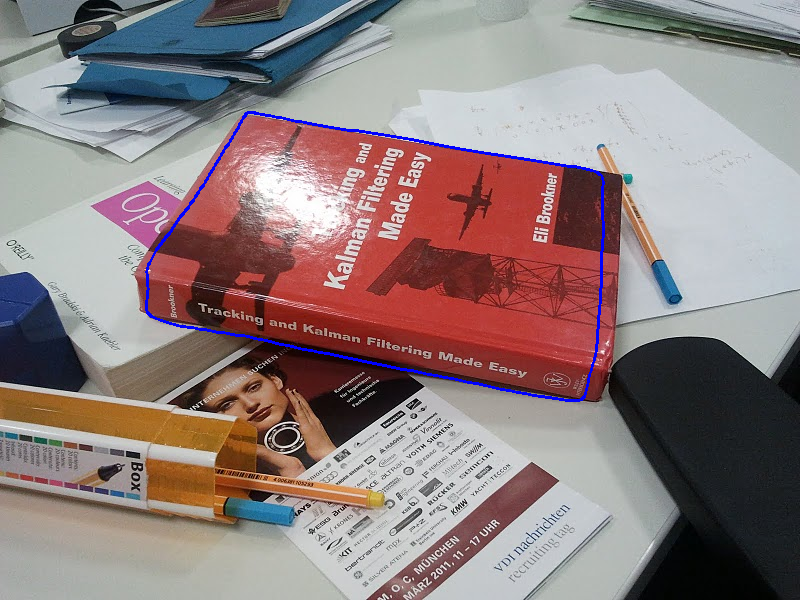
\includegraphics[width=2.0in]{images/book/1.png} 
    \caption{iteration 2} 
    \label{fig:side:b} 
  \end{minipage} 
  \begin{minipage}[t]{0.45\linewidth} 
    \centering 
    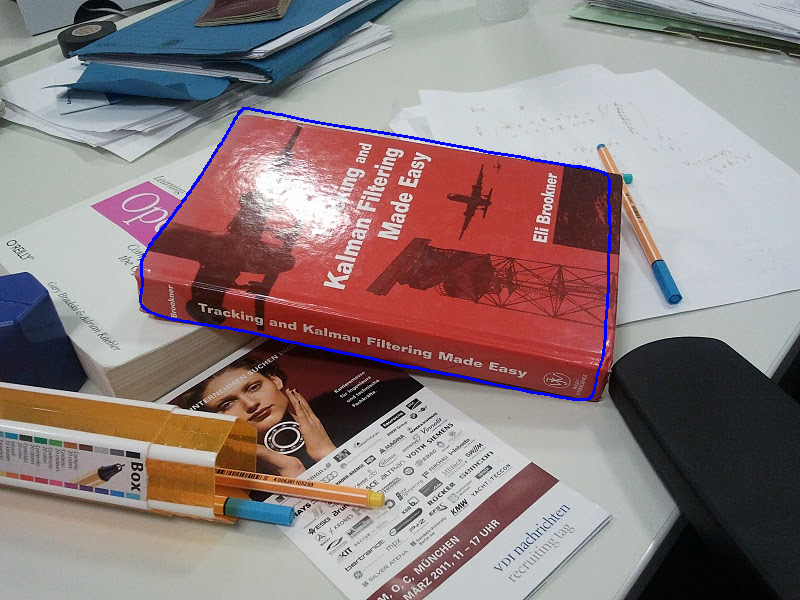
\includegraphics[width=2.0in]{images/book/2.png} 
    \caption{iteration 3} 
    \label{fig:side:c} 
  \end{minipage} 
  \begin{minipage}[t]{0.45\linewidth} 
    \centering 
    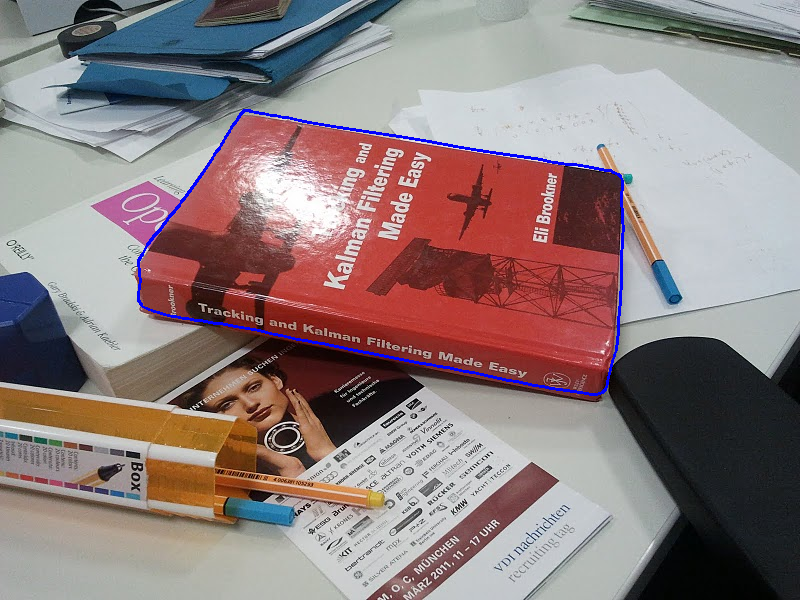
\includegraphics[width=2.0in]{images/book/13.png} 
    \caption{iteration 6} 
    \label{fig:side:d} 
  \end{minipage} 
\end{figure}


\section{Tracking initialization from sift features}
\label{sec:tifsf}

\begin{figure}[htbp]
  \centering
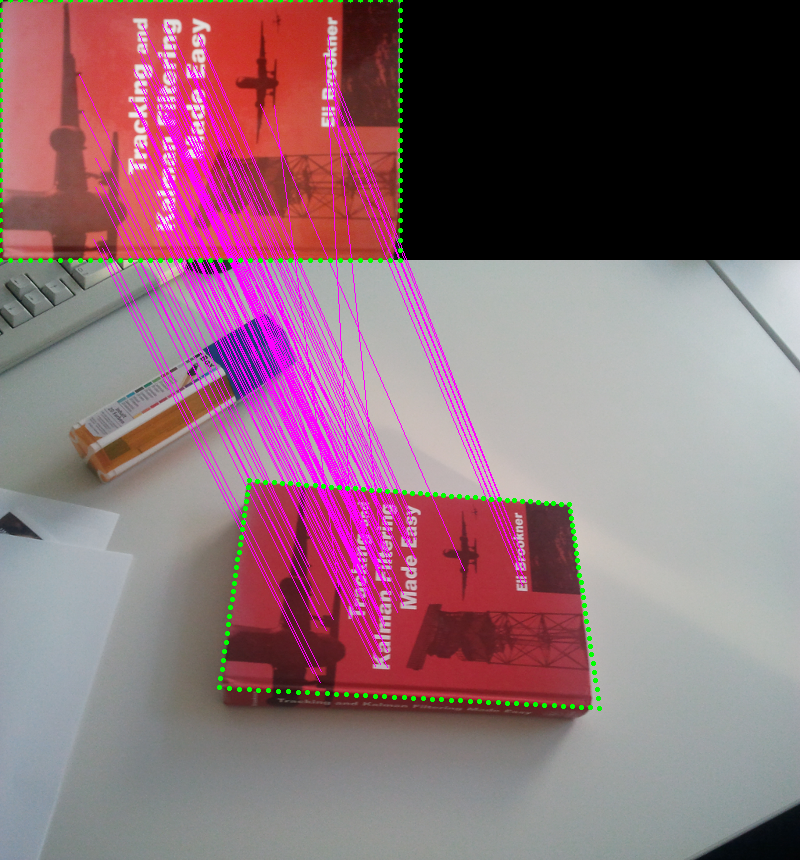
\includegraphics[width=\linewidth]{images/sift.png}
  \caption{sift contour initialization}
  \label{"waiting for reftex-label call..."}
\end{figure}

\begin{figure}[htbp]
  \centering
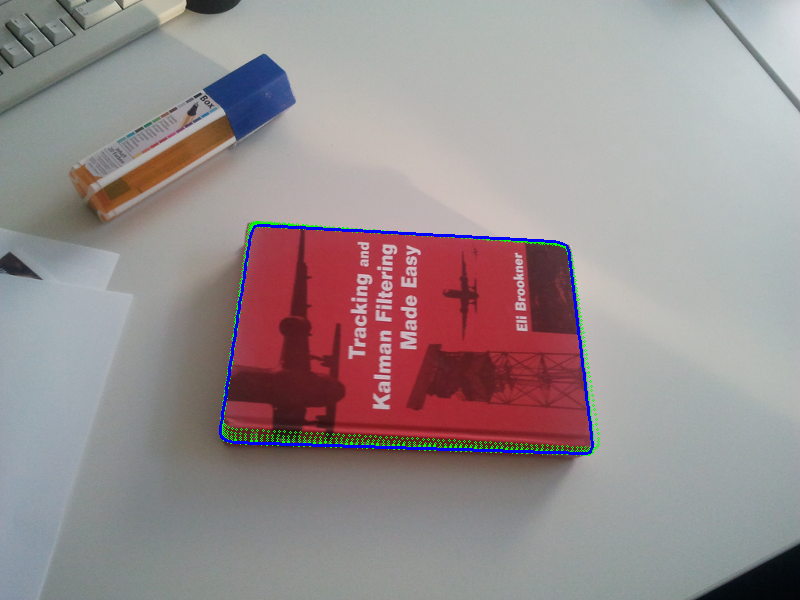
\includegraphics[width=\linewidth]{images/sift_result.png}
  \caption{sift contour initialization}
  \label{"waiting for reftex-label call..."}
\end{figure}


\section{Tracking initialization from 3D point cloud}
\label{sec:tifpc}









